\documentclass{article}
\usepackage[left=1in, right=1in, top=1in]{geometry}
\usepackage[utf8]{inputenc}
\usepackage{amsmath, amssymb, stmaryrd, bm, color}
\usepackage{hyperref}
\usepackage{graphicx}
\graphicspath{ {figures/} }
\usepackage{makecell}
\usepackage{float}
\usepackage{xcolor}
\usepackage{algorithm}
\usepackage{algpseudocode}

\title{Calculating Ellipsoidal Controlled Invariant Sets Using Iterative Inner Approximations}
\author{Tiancheng Ge}
\date{April 2019}

\begin{document}

\maketitle
\tableofcontents

\section{Motivation and Introduction}
Safety is the top concern in self-driving cars. In the field of control and motion planning, we are primarily concerned about designing verifiable safe trajectories that ensure no collision and robustness to disturbances. Nonlinearity and high-dimensionality are the two major challenges.

In this report we focus on dynamical systems with symmetrical properties, and calculate its controlled invariant set using ellipsoidal approximations. For a 5 dimensional nonlinear system, the calculation of ellipsoidal CInvS can be completed in real time (less than a fraction of a second).The control-pre operation can be done at the frequency of about 10 kHz, suggesting that it can be applied to real-time applications, such as calculation of safe set at each time stamp given the previewed disturbances.

The code is open sourced on github
\href{https://github.com/getc1995/ellipsoidal_cinv.git}{https://github.com/getc1995/ellipsoidal\_cinv.git}

\subsection{Literature Review}
For linear systems, \cite{correct-by-construction} calculates polyhedral controlled invariant set (CInvS) offline. During online run time, the controller enforces the states of the system to be inside the controlled invariant set, and that is enough to ensure safety. Polytopic CInvS can be applied to nonlinear systems with some tricks. \cite{lk-cinvs} models the system as a parametric linear system, to handle the non-linear dependency on the longitudinal velocity. The high level idea for calculating CInvS, is to iteratively calculate the control pre set, using polyhedron as the set representation, until the set converges to a CInvS. 

One concern of this method is that the time it takes for the algorithm to converge might be too long. The number of parameter to represent the polyhedral set might increase over the iterations and it is not bounded. This problem is even true when the dimensionality of the system exceeds 5, or the discretized time interval is small (say 0.01 second). However, there are tricks to make the algorithm converge faster, such as cut a small unit ball from the set using Minkowski difference every iteration.
\\

Instead of using polyhedral set representation, other methods, such as control barrier function \cite{control-barrier} and control Lyapunov function \cite{sos-tracking}, use the level set of polynomials to represent the safe set, and sum of square programming are used to optimize the set. Using polynomial representations, these methods are able to handle non-linearity inherently. However, there are problems due to SOS as well:
\begin{enumerate}
    \item It is hard to code the SOS program. The equality/inequality constraints of the system usually have to be transferred into SOS programs manually. SOS programming can handle polynomials pretty well, but for non-linear functions such as sines and cosines, sometimes people have to find good polynomial approximation manually.
    \item A good initial guess is required to run the program. Sometimes there are many constraints on the system, and it is very hard to find a valid initial guess. Also, there is no guarantee that the control barrier/Lyapunov function exists for the given system and the set of safety constraints, and one may continue waste time to find initial guess. 
    \item Bilinear optimization is hard. To optimize control barrier/Lyapunov function, usually we need to optimize the feedback control and the level set alternatively, and global optimality is not guaranteed.
    \item The program becomes very slow as the dimension grows.
\end{enumerate}

On the contrary, the iterative method in \cite{correct-by-construction} and \cite{lk-cinvs} do not have the problem 1-3.

\subsection{Ellipsoidal Approximation Approach}
I would like to utilize the advantages of iterative method to calculate the controlled invariant set, while trying to make the algorithm run faster, by using level set of polynomial instead of the polyhedral set representation. The major problem of polyhedral representation is that the number of parameters in it is unbounded. Only by fixing the number of parameters to represent a set, can we bound the run time for each control-pre set calculation. However, as we fix the number of parameters, we have to do some approximation, because level set of polynomials are not closed under operations like intersection, union, Minkowski sum/difference.\\

One simplest semialgebric set is ellipsoid. Compared to polytopic set methods, the ellipsoidal approximation algorithm is more conservative, but the speed boost is significant. Comparing to SOS based method using second order polynomials, ellipsoidal CInvS method is significantly better in terms of both run time and the size of the set.\\

Instead of using ellipsoidal approximation, it is possible to use higher order polynomial level set, and that could be a good direction to look into. However, the runtime may not be as fast as ellipsoidal approximation, and it may be more tedious to derive closed-form expressions for set approximations.

\section{Preliminaries}

\subsection{Discrete affine dynamical system}
Given a discrete affine dynamical system in the form, $x \in \mathbb{R}^n$ is the state of the system,
$$
\Sigma: x(t+\Delta t) = f[x(t), u(t), d_m(t), d_{um}(t)] =  Ax(t) + Bu(t) + F + E_m d_m(t) + E_{um} d_{um}(t)
$$

where $u$ is the control vector, $d_m$ is the measurable disturbance vector (can be measured by sensor directly or indirectly), $d_{um}$ is the unmeasurable vector (it cannot be measured or it is some sensor noise). We assume $A$ is a non-singular square matrix.\\

If the set of possible control $\mathcal U$, measurable disturbance $\mathcal D_m$ and unmeasurable disturbance $\mathcal D_{um}$ are symmetrical sets about the origin, and $F = \mathbf{0}$,  then we say that the system has symmetric property. \\

A controlled invariant set $\mathcal C$ is a set of $x$ such that
$$
\forall x \in \mathcal C \;\; \forall d_m \in \mathcal D_m \;\; \exists u \in \mathcal  U\;\; \forall d_{um} \in \mathcal D_{um}, \;\;  f(x, u, d_m, d_{um}) \in \mathcal C
$$

Let $\mathcal S$ be some arbitrary set of state $x$ of system $\Sigma$. The control pre set of $\mathcal S$ is defined as 
\begin{equation}
Pre_{\Sigma}(S) := \{\; x \; | \;\;\forall d_m \in \mathcal{D}_m \;\; \exists u \in \mathcal U\;\; \forall d_{um} \in \mathcal D_{um} \;\; \text{s.t.} \;\;  f(x, u, d_m, d_{um}) \in S\;\}
\label{control-pre-def}
\end{equation}

\subsection{Minkowski sum and difference}
The Minkowski sum of two sets $\mathcal{S}_1$ and $\mathcal{S}_2$ with the same dimension $n$ is defined as 
$$
\mathcal{S}_{\text{sum}} = \mathcal{S}_1 \oplus \mathcal{S}_2 = \bigcup_{p_2 \in \mathcal{S}_2} (\mathcal{S}_1 + p_2)
$$
where the $+$ operator for a set and a vector is the overloaded, representing the translation of a set by this vector. The union operation implies $\exists$, and $\mathcal{S}_{\text{sum}}$ is a set such that

$$
\forall x \in \mathcal S_{\text{sum}} \;\;\exists p_2 \in \mathcal{S}_2  \;\;\exists p_1 \in \mathcal{S}_1, x =  p_1 + p_2
$$

The Minkowski difference of two sets $\mathcal{S}_1$ and $\mathcal{S}_2$ with the same dimension $n$ is defined as 
$$
\mathcal{S}_{\text{diff}} = \mathcal{S}_1 \ominus \mathcal{S}_2 = \bigcap_{p_2 \in \mathcal{S}_2} (\mathcal{S}_1 + p_2)
$$

The intersect operation implies $\forall$, and $\mathcal{S}_{\text{diff}}$ is a set such that
$$
\forall x \in \mathcal S_{\text{diff}}  \;\;\forall p_2 \in \mathcal{S}_2 \;\;\exists p_1 \in \mathcal{S}_1, x = p_1 + p_2 
$$

For a linear time invariant system $\Sigma$, the control pre set of $\mathcal{S}$ can be calculated by 

\begin{equation}
Pre_{\Sigma}(S) = A^{-1}\left[S \ominus E_{um} \mathcal D_{um} \oplus B \mathcal U \ominus E_{m} \mathcal D_{m}\right]
\label{control-pre}
\end{equation}

The order of Minkowski difference first, Minkowski sum second and Minkowski difference last corresponds to the order of ($\forall d_{um}, \exists u, \forall d_{m}$) in the definition of control pre set in Def. \ref{control-pre-def}.

In \cite{ellipsoid-toolbox}, there is formula for forward reachable set in Minkowski sum/difference form.

To calculate polytopic control pre set, the Minkowski sum operation is implemented as projection, and the Minkowski difference operation is implemented as intersection.\\

For most application in robotics or specifically self-driving cars, the set of disturbance and control are usually hyperrectangles, and $E_{um} \mathcal D_{um}, B \mathcal U, E_{um} \mathcal D_{um}$ are parallelotopes (degenerated or non-degenerated). Also, the safety constrain is usually symmetrical about the origin as well. (For ACC, the headway could go to positive infinity, but let's say we want to constrain the headway in some interval center around the desired headway.)

In this report, I primarily consider using ellipsoids to represent the set of state $x$ of the system with symmetric property, and treat set of control/disturbance as hyperrectangles.

\section{Linear Systems with Symmetric Properties}

\subsection{Algorithms}
Now let's try to calculate an ellipsoidal CInvS of a linear system $\Sigma$ using control pre operations. For safety concerns, we would like to calculate an inner approximation of the control pre set of an ellipsoidal set. 

Using Eqn. \ref{control-pre} and the inner approximation algorithms for Minkowski sum/difference of an ellipsoid and a parallelotope described in the ellipsoidal approximation report, we should be able to calculate the control pre (backward reachable set). Here is the algorithm:

\begin{algorithm}[H]
	\centering
	\caption{Calculate control pre set of a ellipsoidal set $\mathcal E := \{x\;|\;(x-c)^T E (x-c) \leq 1\}$, for system $\Sigma$}
\begin{algorithmic}[1]
	\Function{pre}{$\Sigma, \mathcal E$}
	\State{$\mathcal E \leftarrow$  Minkdiff\_ia($\mathcal E, \Sigma.E_{um} \mathcal D_{um}$)}
	\State{\textbf{if} $\mathcal E$ is $\emptyset$}
	\State\hspace{\algorithmicindent}{\textbf{return} $\emptyset$}
	\State{$\mathcal E \leftarrow$ Minksum\_ia($\mathcal E, \Sigma.B \mathcal U$)}
	\State{$\mathcal E \leftarrow$ Minkdiff\_ia($\mathcal E, \Sigma.E_{m} \mathcal D_{m}$)}
	\State{\textbf{if} $\mathcal E$ is $\emptyset$}
	\State\hspace{\algorithmicindent}{\textbf{return} $\emptyset$}
	\State{$\mathcal E.E \leftarrow (\Sigma.A)^T(\mathcal E.E) (\Sigma.A)$}
	\State{$\mathcal E.c \leftarrow (\Sigma.A)^{-1}(\mathcal E.c)$}
	\State{\textbf{return} $\mathcal E$}
	\EndFunction
\end{algorithmic}
\label{alg_pre}
\end{algorithm}

Alg. \ref{alg_pre} pre function should return an empty set or warning if the control pre set of the input ellipsoidal set is empty.

Then, we can use pre operation to calculate the ellipsoidal CInvS. The following algorithm is similar to inside-out/outside-in algorithm, but there are some differences.
 
\begin{algorithm}[H]
	\centering
	\caption{Calculate CInvS of system $\Sigma$, given inequality constraint $Ax \leq b$}
	\begin{algorithmic}[1]
		\Function{getCInvS}{$\Sigma, A, b$}\\
		Assume that system $\Sigma$ has symmetric property, and the box constraint is symmetric as well.
		\State{$\mathcal C \leftarrow$ Some ellipsoid centered at the origin and contained in polytope $\{x\;| Ax \leq b\}$}
		\State{\textbf{while} True}
		\State\hspace{\algorithmicindent}{$\mathcal C_{\text{pre}} \leftarrow$ pre($\Sigma, \mathcal C$)}
		\State\hspace{\algorithmicindent}{\textbf{if} $\mathcal C_{\text{pre}}$.contains($\mathcal C$) }% and $(\mathcal C_{\text{pre}}.\text{volume} - \mathcal C.\text{volume} < \text{tolerance} \;\;\epsilon)$
		\State\hspace{\algorithmicindent}\hspace{\algorithmicindent}{\textbf{break}}
		\State\hspace{\algorithmicindent}{Find the inscribed ellipsoid inside the intersection of $\mathcal C_{\text{pre}}$ and polytope $\{x\;| Ax \leq b\}$}
		\State\hspace{\algorithmicindent}{$\mathcal C \leftarrow$ intersect($\mathcal C_{\text{pre}}, A, b$)}
		\State{\textbf{return} $\mathcal C$}
		\EndFunction
	\end{algorithmic}
	\label{alg_cinvs}
\end{algorithm}

For outside-in algorithm, in each iteration, $\mathcal C \leftarrow \mathcal C \bigcap \mathcal C_{\text{pre}}$, so the volume of $\mathcal C$ is strictly decreasing.

For inside-out algorithm, $\mathcal C$ is initialized to some controlled invariant set of the system, and in each iteration, $\mathcal C \leftarrow \text{polytope}(A,b) \bigcap \mathcal C_{\text{pre}}$, and the volume of $\mathcal C$ is strictly increasing.\\

In my proposed algorithm, $\mathcal C$ is initialized to some arbitrary large enough set, not necessarily a CInvS, like the outside-in algorithm. However, it is using an update rule similar to inside-out. 

I postulate that when calculating polytopic controlled invariant set, even if the set $\mathcal C$ is not initialized to some CInvS, the algorithm will eventually converge to a CInvS, but in practice it may take a long time.

I postulate that the proposed algorithm will converge if there exists a ellipsoidal CInvS for the given system and safety constraints.

Two points to note in Alg. \ref{alg_cinvs}:
\begin{enumerate}
\item For inside-out, the update rule $\mathcal C \leftarrow \text{polytope}(A,b) \bigcap \mathcal C_{\text{pre}}$ directly takes the intersection. In the proposed algorithm, we check if $\mathcal C_{\text{pre}}$.contains($\mathcal C$) before doing the intersection. This is because the ellipsoidal approximation of $\text{polytope}(A,b) \bigcap \mathcal C_{\text{pre}}$ may not contains $\mathcal C$, even if $\mathcal C$ is a CInvS. For polytopic sets, the intersection is exact and no approximation is involved, so that doesn't matter.
\item Here the terminating condition is $\mathcal C_{\text{pre}}$.contains($\mathcal C$), which only checks if $\mathcal C$ is a controlled invariant set. Instead of breaking the loop directly after finding a CInvS, one could continue the iteration until the volume converges. However, in practice, the volume converges before $\mathcal C$ becomes a CInvS.
\end{enumerate}

\subsection{Experiments on lane keeping, constant velocity}

Eqn. \ref{eq:lk} describes the lane keeping continuous dynamics. This system is a typical example that has symmetric property.

Here for simplicity, I ignore the inter-sampling behavior and discretize the system anyway. However, the error term introduced by inter-sampling behavior can be modeled as measurable disturbances, using the technique in section \ref{section_nonlinear}.

\begin{equation}
\label{eq:lk}
\frac{\mathrm{d}}{\mathrm{d}t} \begin{bmatrix} y \\ v \\ \Delta \Psi \\ r \end{bmatrix}
=  \underbrace{\begin{bmatrix} 0 & 1 & u & 0 \\
	0 & -\frac{ C_{\alpha f} + C_{\alpha r} }{ mu } & 0 & -\frac{a C_{\alpha f} - b C_{\alpha r}}{ mu } - u \\
	0 & 0 & 0 & 1  \\
	0 & -\frac{a C_{\alpha f} - b C_{\alpha r} }{ I_{z} u } & 0 & -\frac{a^2 C_{\alpha f} + b^2 C_{\alpha r} }{ I_{z} u }
	\end{bmatrix}}_{A_{LK}}
\begin{bmatrix} y \\ v \\ \Delta \Psi \\ r \end{bmatrix}
+
\underbrace{\begin{bmatrix} 0 \\ \frac{C_{\alpha f} }{m} \\ 0 \\ a \frac{C_{\alpha f} }{I_{z}} \end{bmatrix}}_{B_{LK}} \delta_f 
+  
\underbrace{\begin{bmatrix} 0 \\ 0 \\ -u \\ 0 \end{bmatrix}}_{E_{LK}} \kappa_{d}
\end{equation}

First, let's consider the case where the longitudinal velocity $u$ is constant. When the polytopic method is able to find a CInvS, the ellipsoidal algorithm usually success as well. \\

After some experiments, the only case in which the ellipsoidal method fails, is that when polytopic CInvS is skewed and ill-conditioned (for example, looks like very thin plane). In this case, the system is very hard to control anyway, and if we increase the disturbance a little bit, the polytopic method cannot find the CInvS as well.

A comparison of the controlled invariant sets found by polytopic and ellipsoidal methods are shown in Table \ref{lk}.

\begin{table}[H]
	\centering
	\begin{tabular}{ccc}
		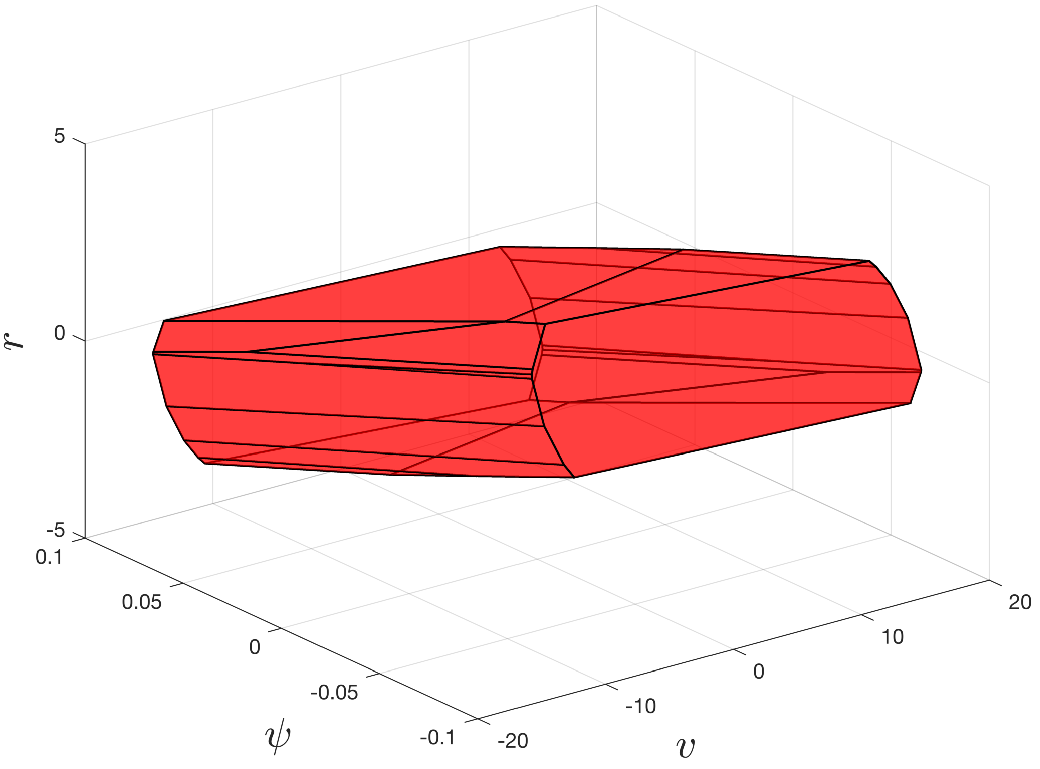
\includegraphics[width=0.3\textwidth]{lk/poly1.pdf} & 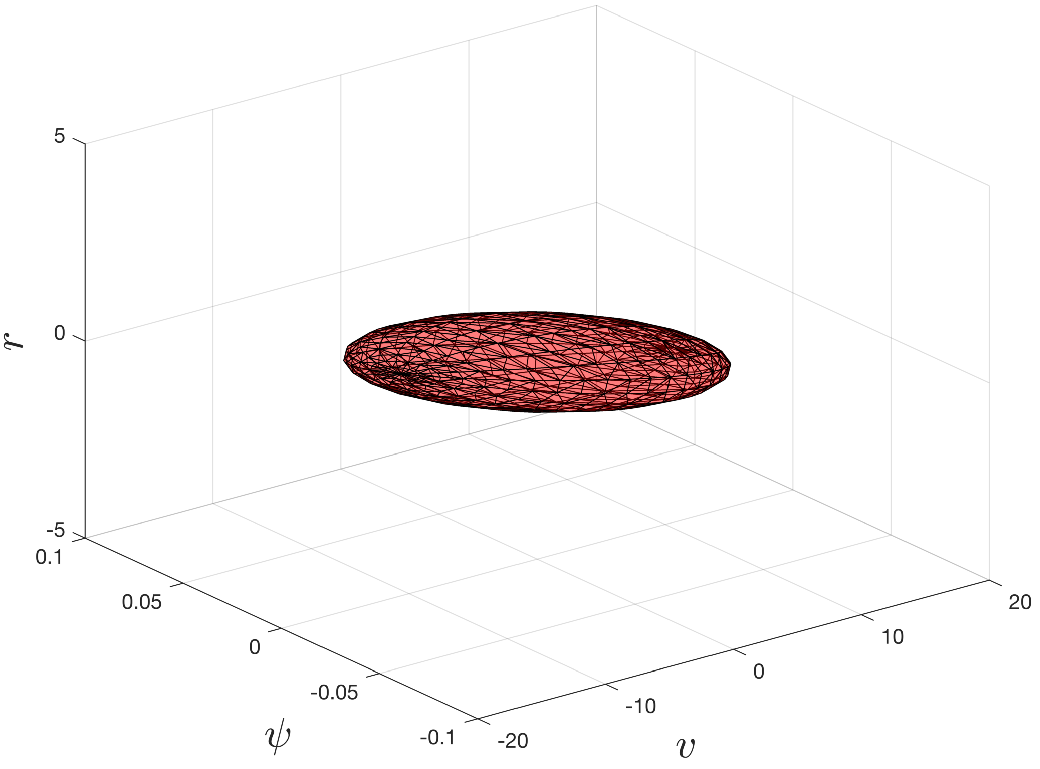
\includegraphics[width=0.3\textwidth]{lk/ellip1.pdf} &
		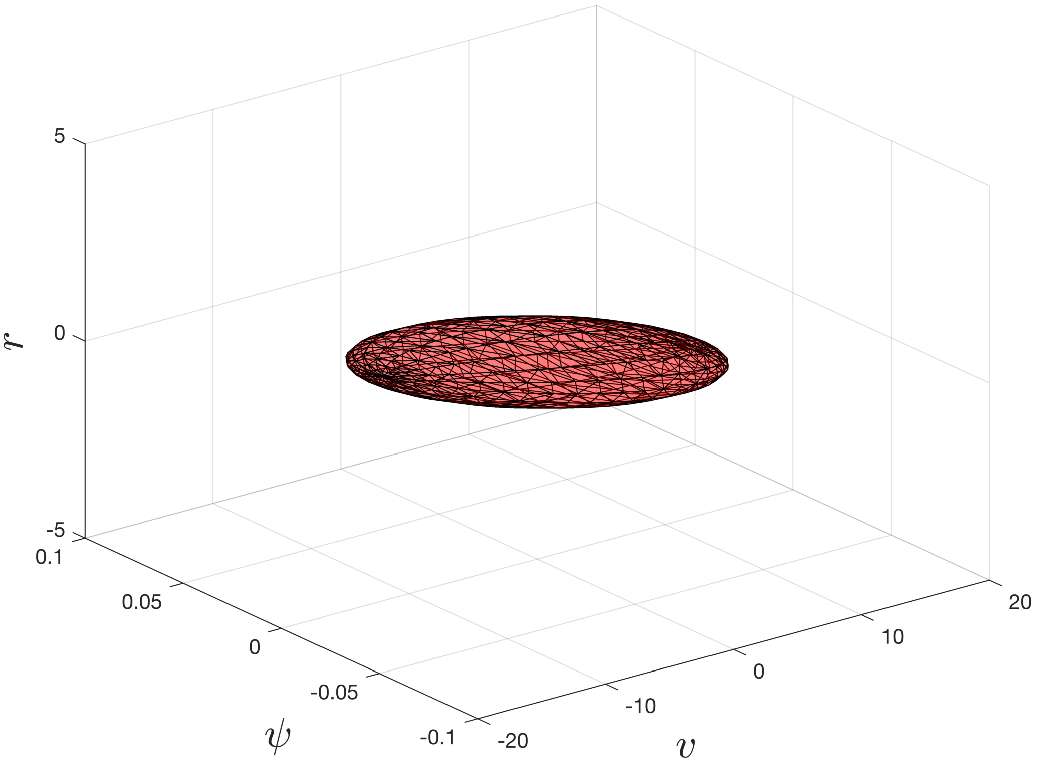
\includegraphics[width=0.3\textwidth]{lk/ellip1_conservative.pdf} \\
		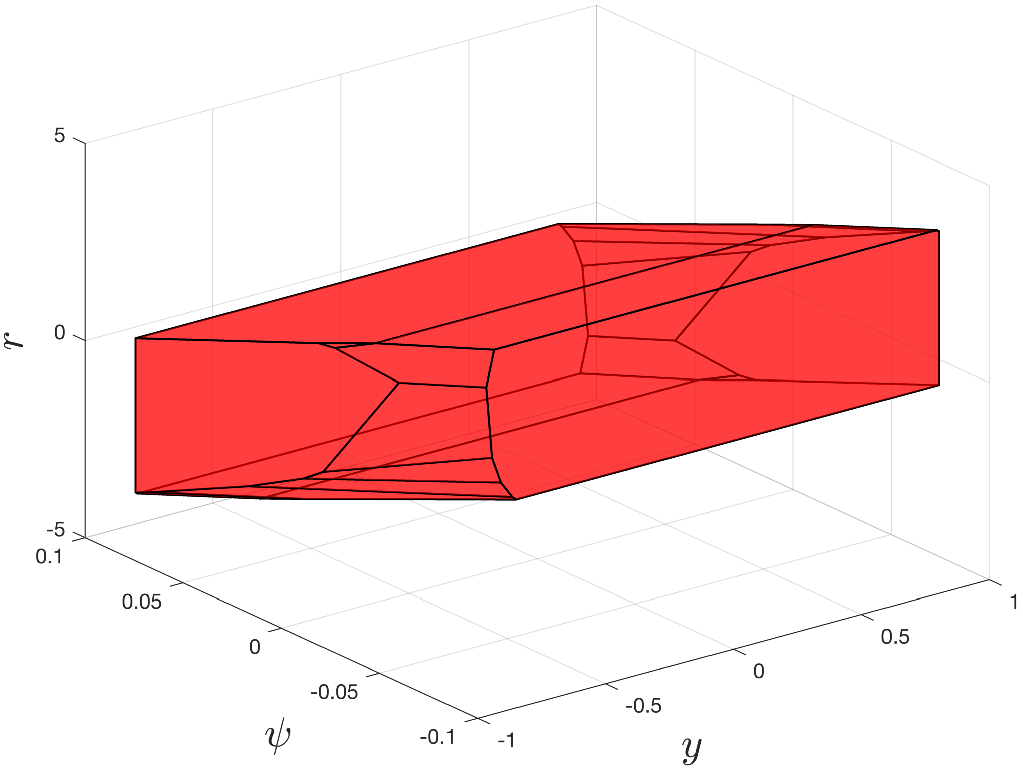
\includegraphics[width=0.3\textwidth]{lk/poly2.pdf} & 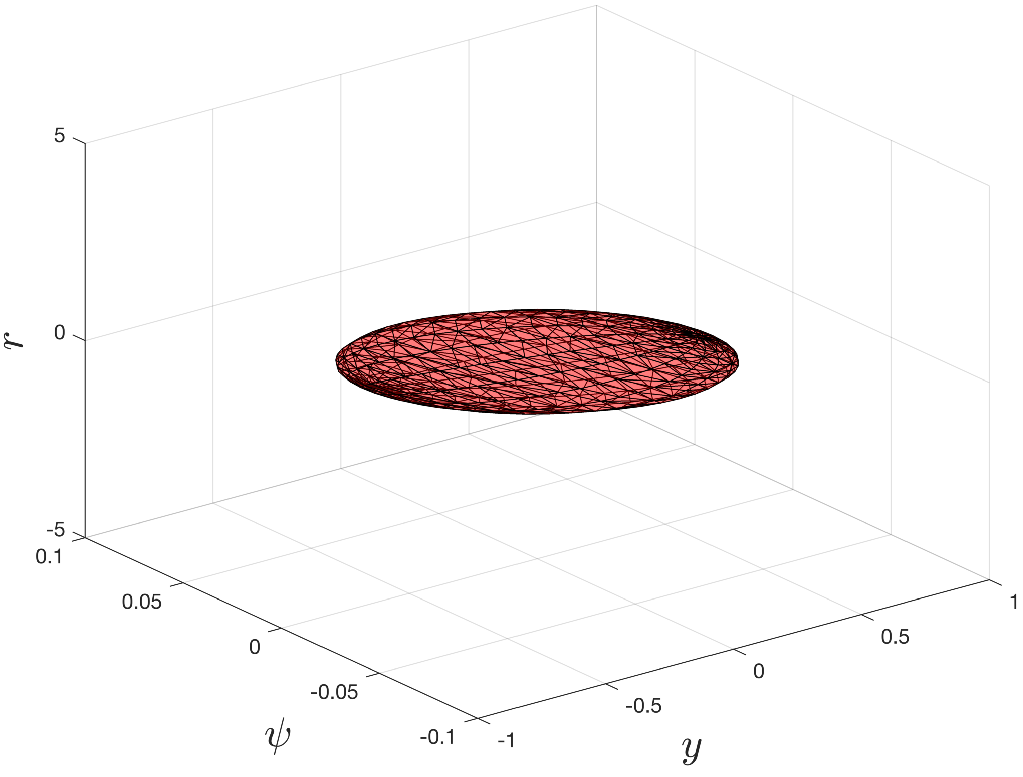
\includegraphics[width=0.3\textwidth]{lk/ellip2.pdf}&
		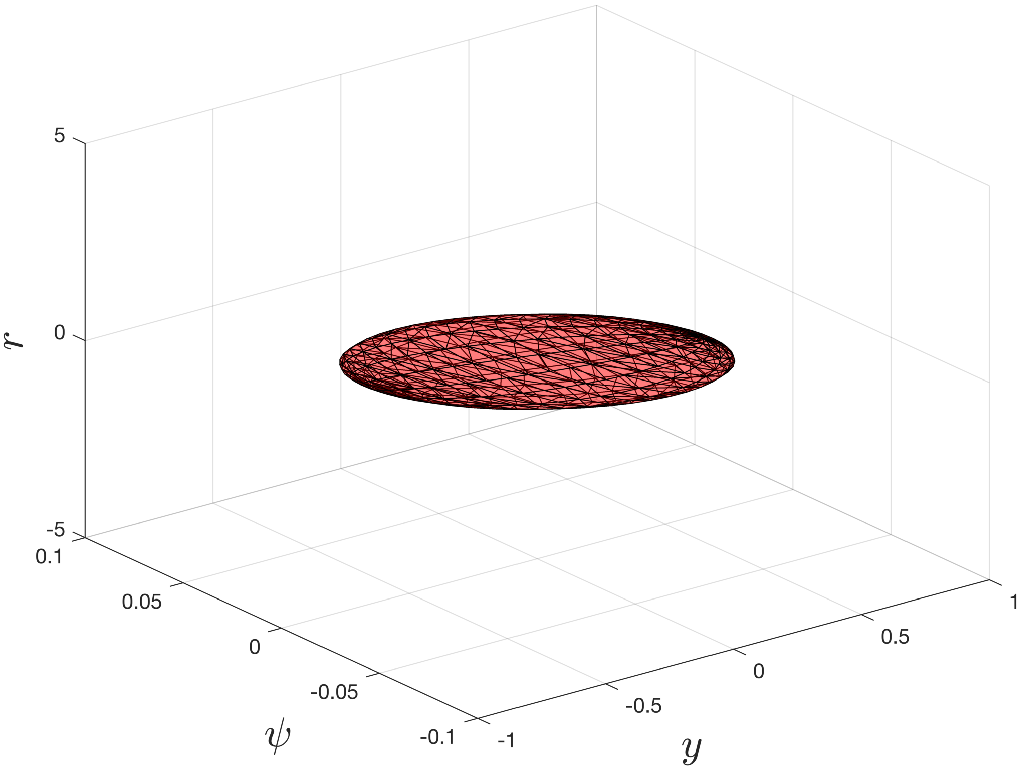
\includegraphics[width=0.3\textwidth]{lk/ellip2_conservative.pdf} \\
		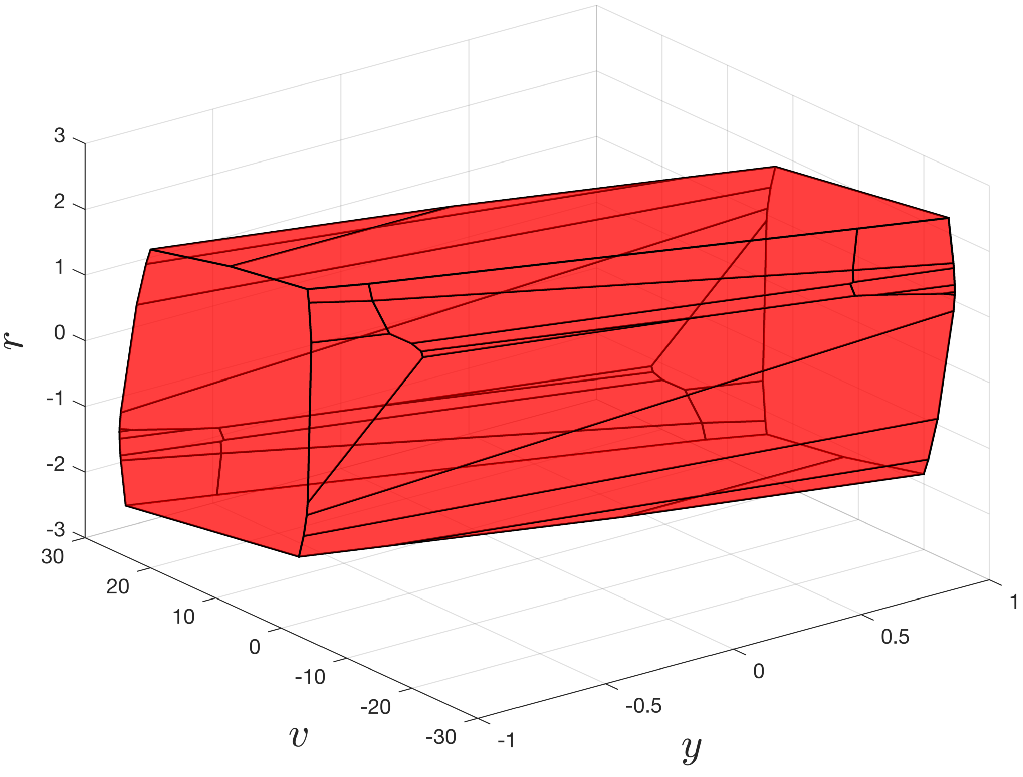
\includegraphics[width=0.3\textwidth]{lk/poly3.pdf} & 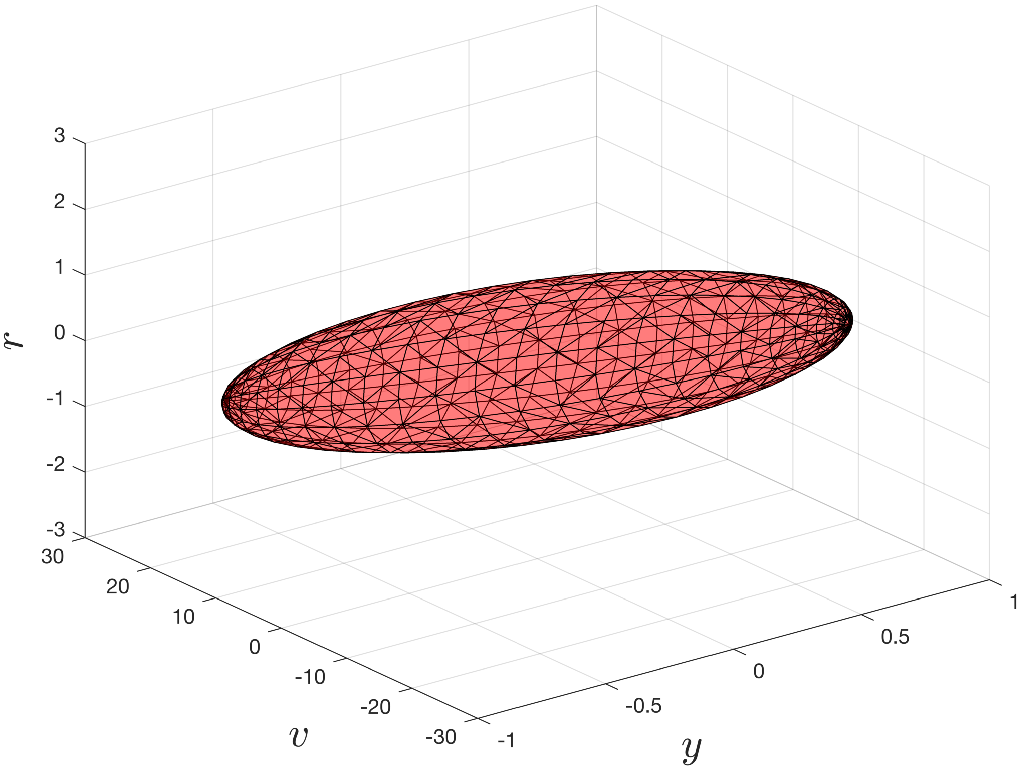
\includegraphics[width=0.3\textwidth]{lk/ellip3.pdf}&
		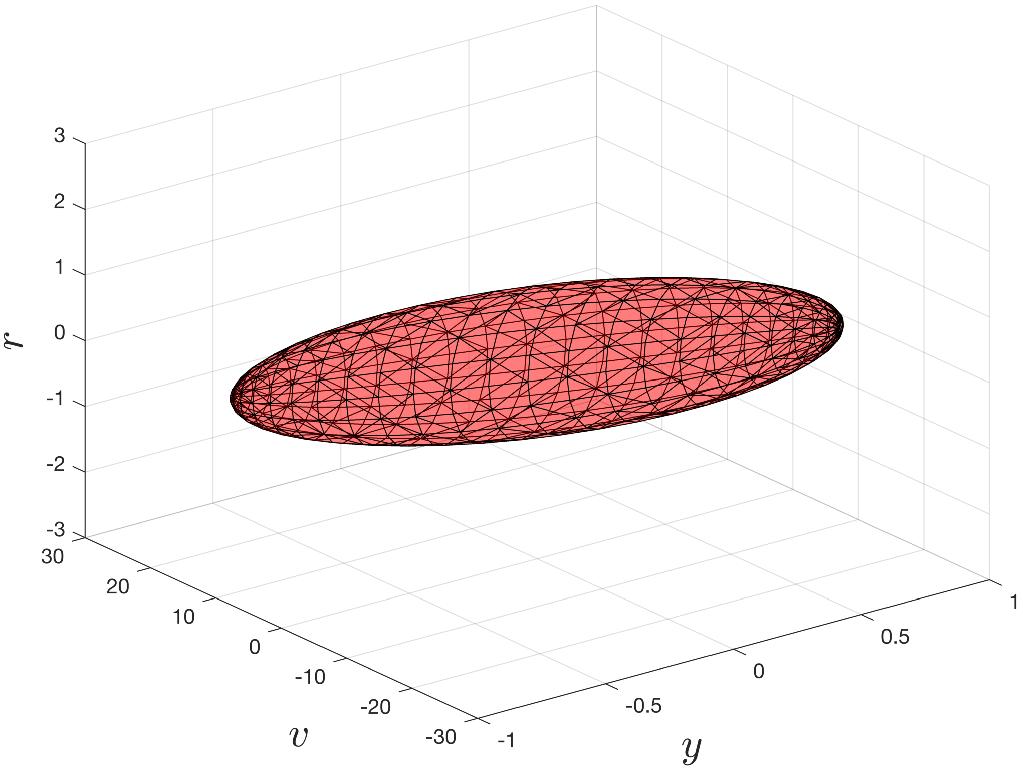
\includegraphics[width=0.3\textwidth]{lk/ellip3_conservative.pdf} \\
		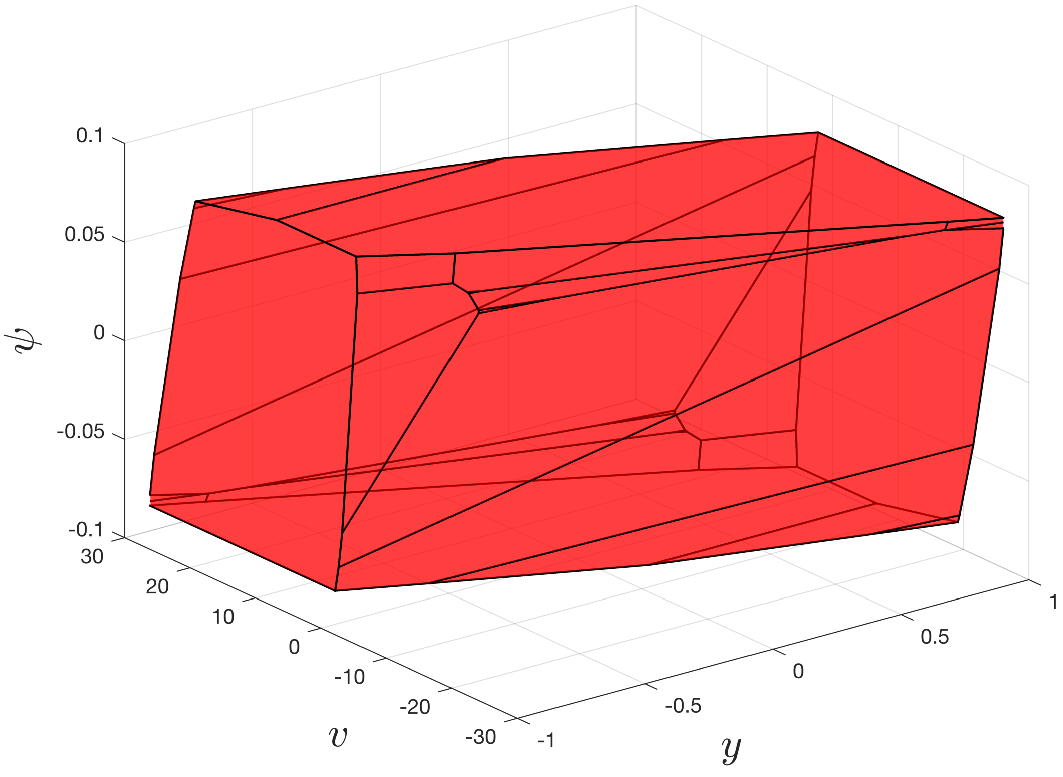
\includegraphics[width=0.3\textwidth]{lk/poly4.pdf} & 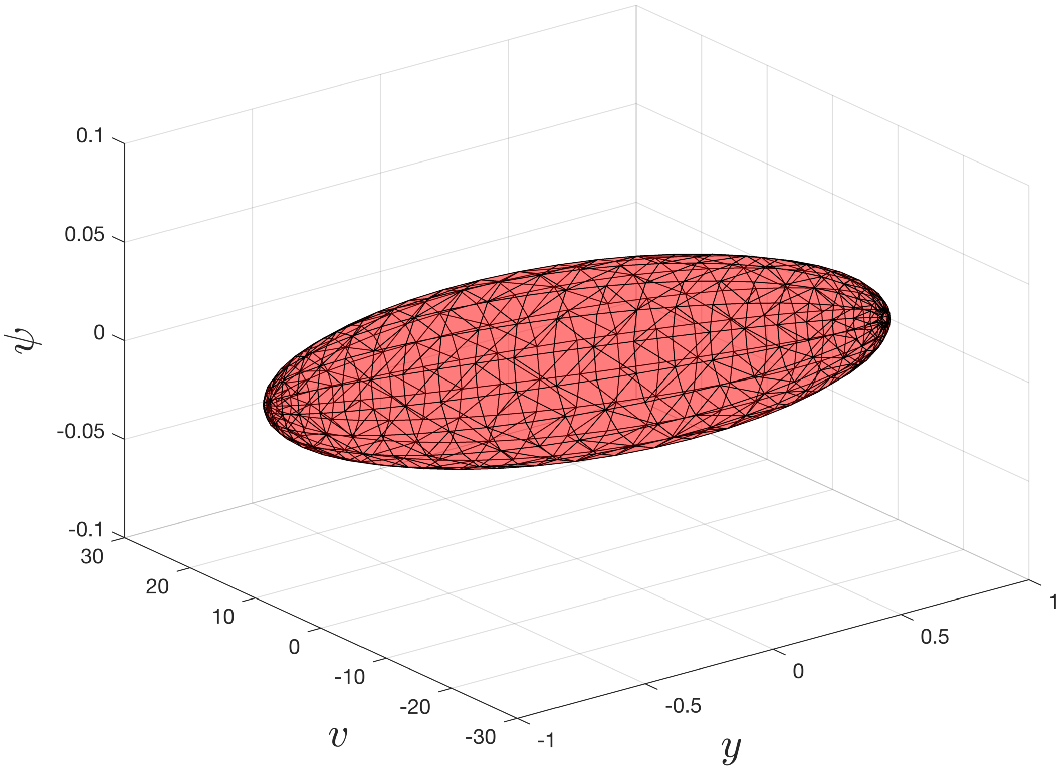
\includegraphics[width=0.3\textwidth]{lk/ellip4.pdf}&
		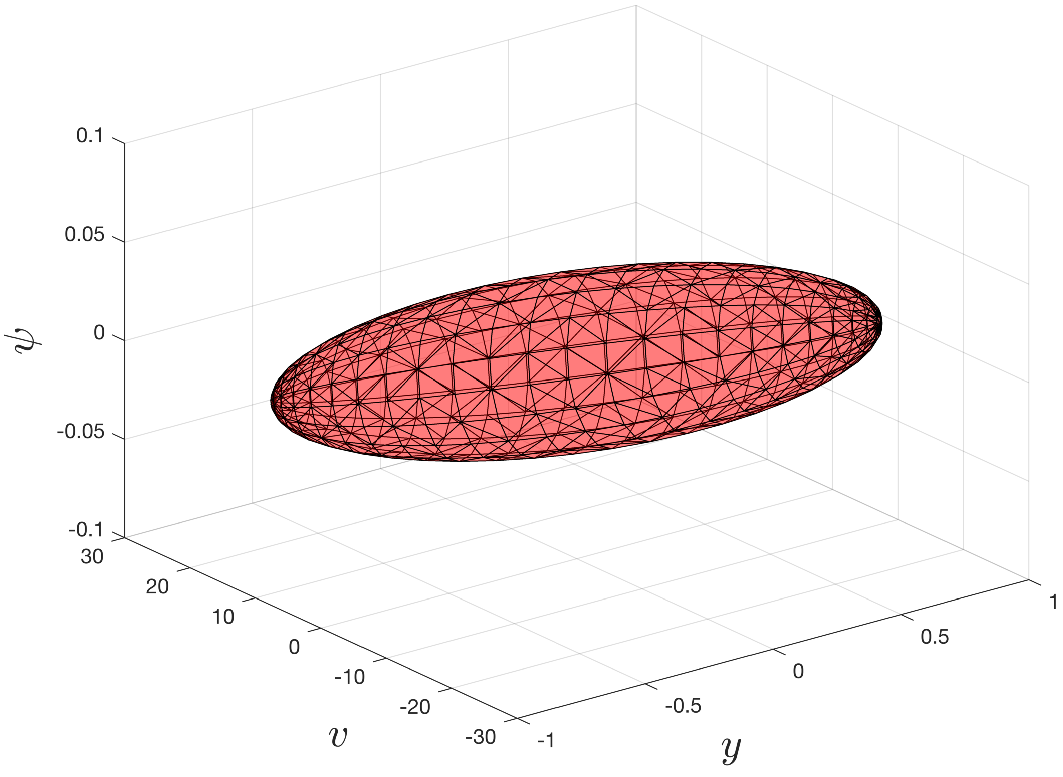
\includegraphics[width=0.3\textwidth]{lk/ellip4_conservative.pdf} \\
	\end{tabular}
	\caption{The polytopic and ellipsoidal CInvS for 4D lane keeping system, intersect with the plane $y=0, v=0, \Psi=0$ and $r=0$, respectively. The volume of the ellipsoidal CInvS is  less than the polytopic one, but their size in each dimension is still at the same order of magnitude. The third column is the ellipsoidal set calculated by the modified algorithm.}
	\label{lk}
\end{table}

\begin{table}[H]
	\centering
	\begin{tabular}{|l|c|c|c|}
		\hline
		&  \makecell{Polytopic \\zero $d_{um}$} &  \makecell{Ellipsoidal \\zero $d_{um}$} & \makecell{Ellipsoidal \\nonzero $d_{um}$}\\
		\hline
		$\Delta t = 0.1$s & 2.36 s & 0.09 s & 0.16 s\\
		$\Delta t = 0.01$s & N/A s & 0.54 s & 0.80 s\\
		$\Delta t = 0.001$s & N/A s & 3.96 s & 5.68 s\\
		$\Delta t = 0.0001$s & N/A s & 33.99 s & 47.50 s\\
		\hline
	\end{tabular}
	\caption{Run time for each algorithm with different $\Delta t$. For ellipsoidal methods, the run time increases inverse-proportionally to $\Delta t$.}
	\label{lk_runtime}
\end{table}

When doing online control with quadratic cost, plus the constraint that the states should always be inside the ellipsoidal CInvS, we can write this optimal control problem into a convex QCQP (Quadratically constrained quadratic program). 
\begin{enumerate}
\item Assume no ummeasurable disturbances, and the ellipsoidal CInvS is in the form of $\{x\;| \; x^T E x \leq 1\}$. The QCQP can be written as
\begin{align*}
\text{argmin}_{u(1), \dots, u(T)}  \quad & \sum_{t=0}^T \left(\begin{bmatrix}x(t)^T u(t)^T \end{bmatrix} W \begin{bmatrix}x(t) \\u(t) \end{bmatrix}\right)\\
\text{subject to} \quad & x(t)^T E x(t) \leq 1 \;\;\text{for}\;\; t = 1, \dots, T\\
& x(t) = Ax(t-1) + Bu(t) + E_m d_m\;\;\text{for}\;\; t = 1, \dots, T\\
& x(0) = x_0
\end{align*}

At each time stamp, we solve this QCQP. In fact, to sure safety, the ellipsoidal CInvS constraint only need to be enforced at $t=1$.

\item When there are ummeasurable disturbances, let the ellipsoidal set $\{x\;| \; x^T E x \leq 1\}$ be the inner approximation of CInvS $\ominus E_{um} \mathcal D_{um} $, instead of CInvS itself.
\end{enumerate}

The QCQP can be solved by general solvers like CVX, but they are not specialized for QCQP and they are very slow. Luckily, QCQP can be manually written into second-order cone program (SOCP) with linear objective function \cite{convexopti}, and can be solved very fast by specialized solver, such as ECOS \cite{ecos}. For this 4 dimensional lane keeping system with 20 time step horizon, the SOCP solver can run at 300 Hz, which is fast enough for real time application.

\begin{figure}[H]
	\centering
	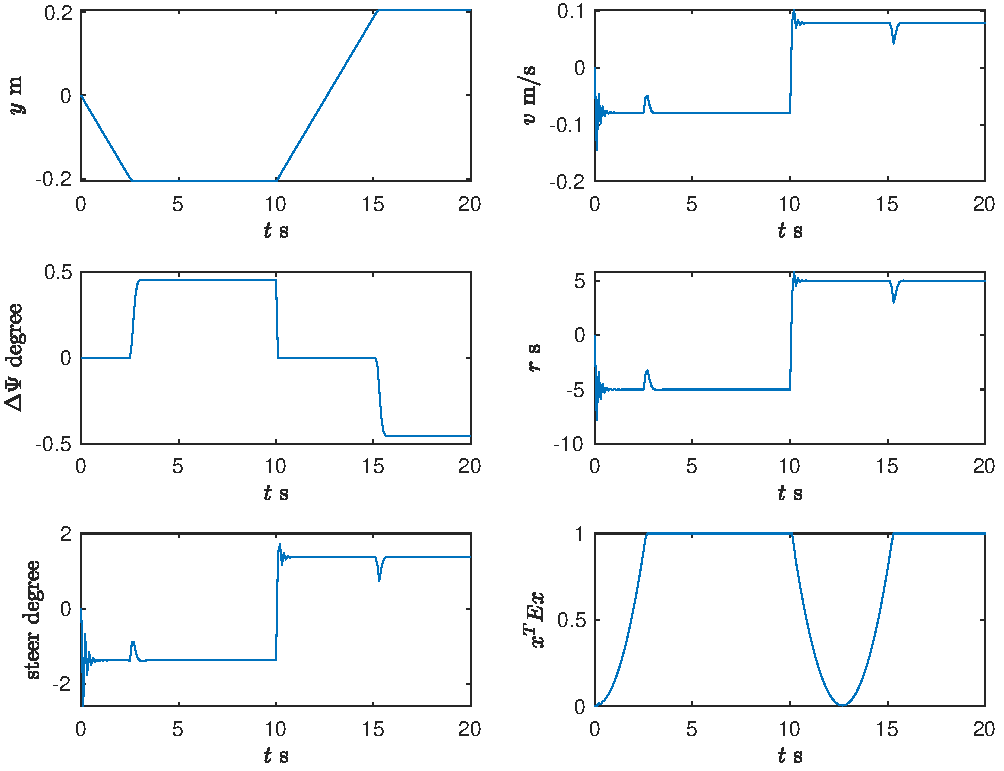
\includegraphics[width=0.8\linewidth]{lk/step_response.pdf}
	\caption{$x(0) = \mathbf{0}$. $ d_{m}(t) = -5 \; \mathrm{degree/s}, t \in [0,10)$. $d_{m}(t) = 5  \;\mathrm{degree/s}, t \in [10,20] $. Using a QCQP controller with controlled invariant set constraint only at the first timestamp, although the cost function only penalize the yaw rate $r$, the controller is able to satisfy the safety constraint. $x^T E x$ is always within [0, 1], meaning that the states never violate the controlled invariant set.}
	\label{lk_step_response}
\end{figure}


\subsection{Experiments on lane keeping, velocity band}
Here let's take the longitudinal velocity $u$ as a parameter, and $u \in [u_1, u_2]$. Use the algorithm from \cite{lk-cinvs}, we can find the convex hull of the system parameterized over $u$, and take the intersection of control pre sets of all the systems at the vertex of the convex hull.

As discussed in the Ellipsoidal approximation report, the current algorithm used to do the inner approximation of multiple ellipsoids (over two) is not optimal. Never the less, we are still able to find ellipsoidal CInvS for a velocity band. Table \ref{lk_band_runtime} shows the runtime of the algorithm. Figure \ref{lk_vband_step_response} shows the simulated system with the QCQP controller.

\begin{table}[H]
	\centering
	\begin{tabular}{|c|c|}
		\hline
		$\Delta t$ &  runtime \\
		\hline
		$0.1$s & 0.14 s \\
		$0.01$s & 0.46 s \\
		$0.001$s & 2.81 s \\
		$0.0001$s & 23.07 s \\
		\hline
	\end{tabular}
	\caption{Run time for the algorithm with different time discretization $\Delta t$. The run time increases inverse-proportionally to $\Delta t$.}
	\label{lk_band_runtime}
\end{table}

\begin{figure}[H]
	\centering
	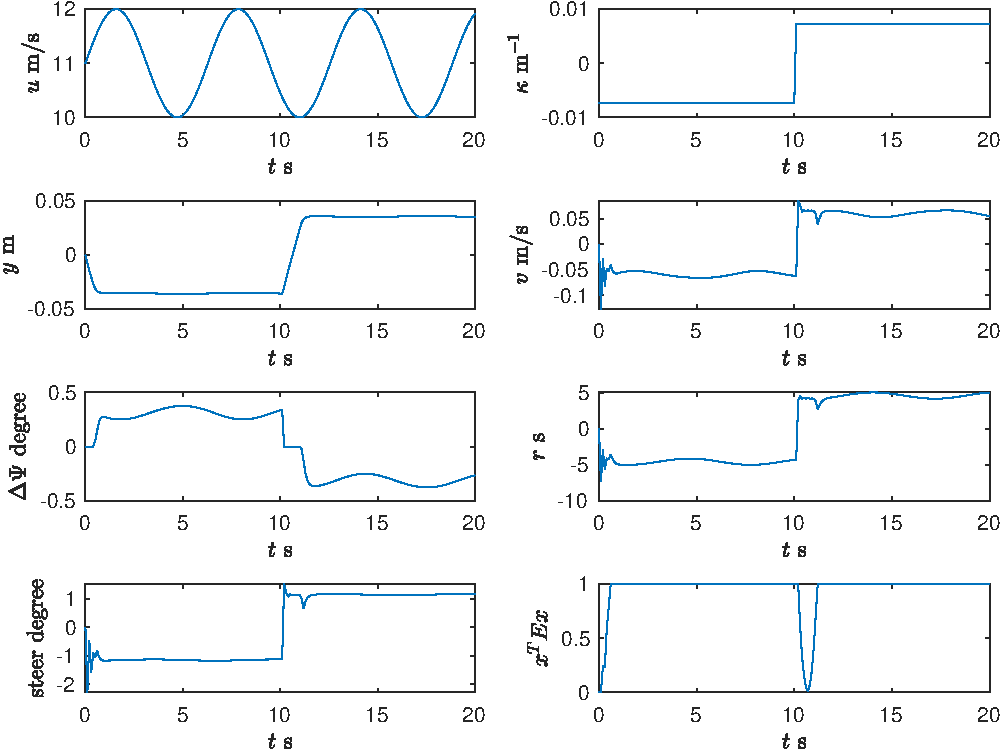
\includegraphics[width=0.8\linewidth]{lk_vband/step_response.pdf}
	\caption{Experiment on varying longitudinal velocity. Using a QCQP controller with controlled invariant set constraint only at the first timestamp, although the cost function only penalize the yaw rate $r$, the controller is able to satisfy the safety constraint. $x^T E x$ is always within [0, 1], meaning that the states never violate the controlled invariant set.}
	\label{lk_vband_step_response}
\end{figure}


\subsection{Handling preview}
The runtime for calculate an ellipsoidal control pre set is very fast, and it can run at 10kHz for 4 dimensional lane keeping system. It becomes possible to calculate the backward reachable set based on previewed measurable disturbances. Alg. \ref{alg_pre_preview} illustrates the procedure to calculate the backward reachable set.

Having the backward reachable set, which looks like a funnel, the state of the system doesn't have to be maintained inside the CInvS all the time. It is enough to maintain the states inside the backward reachable set.

\begin{algorithm}[H]
	\centering
	\caption{Calculate control pre set of a ellipsoidal set $\mathcal E := \{x\;|\;(x-c)^T E (x-c) \leq 1\}$ with previewed disturbance $d_m$, for system $\Sigma$. This control pre set also has to be inside polytopic constraint $\{x\;| \; Ax \leq b \}$}.
	\begin{algorithmic}[1]
		\Function{pre\_preview}{$\Sigma, \mathcal E, d_m, A, b$}
		\State{$\mathcal E \leftarrow$  Minkdiff\_ia($\mathcal E, \Sigma.E_{um} \mathcal D_{um}$)}
		\State{\textbf{if} $\mathcal E$ is $\emptyset$}
		\State\hspace{\algorithmicindent}{\textbf{return} $\emptyset$}
		\State{$\mathcal E \leftarrow$ Minksum\_ia($\mathcal E, \Sigma.B \mathcal U$)}
		\State{$\mathcal E.c \leftarrow$ $\mathcal E.c - d_m$ }\\
		\State{$\mathcal E.E \leftarrow (\Sigma.A)^T(\mathcal E.E) (\Sigma.A)$}
		\State{$\mathcal E.c \leftarrow (\Sigma.A)^{-1}(\mathcal E.c)$}
		\State{$\mathcal E \leftarrow$ intersect($\mathcal E, A, b$)}
		\State{\textbf{return} $\mathcal E$}
		\EndFunction
	\end{algorithmic}
	\label{alg_pre_preview}
\end{algorithm}

\textcolor{red}{TODO: For now, if the ellipsoid is not centered at the origin, the algorithm that finds the intersection of the ellipsoid  and a symmetrical box is not implemented, because the close-form solution is more complex and non-trivial to derive.}

\subsection{Problems in evaluating conservatism}
\begin{enumerate}
	\item Curse of dimensionality. Is volume a good metric for evaluating the conservatism of a safe set?
	
	In general, we want the safe set to be as large as possible. Smaller safe set is more conservative (less space to move around and minimizing jerk). Volume is usually used to measure how large a set is. However, when the dimension of a unit ball increases, the volume within 90\% of its radius decreases.
	
	Denote the volume of a hyper dimensional ball as $V$, and denote the volume within 95\% of its radius as $V_{90\%}$.
	
	$$
	\frac{V_{9\%}}{V} = \left(\frac{0.9r}{r}\right)^n = 0.9^n
	$$
	
	For 4 dimensional system, $n=4$ and  $\frac{V_{9\%}}{V} = 0.65$, meaning that there are 35\% of volume is in the shell that outside 90\% of the radius. Intuitively, the state of the system wouldn't be inside the shell for too long.
	
	An alternative is using trace of the determinant, and that is related to the length of each principle semi-axis. But still, we don't know which axis of the ellipsoidal set matters most, since they could represent different physical quantities (velocity, yaw rate, headway, etc.).
	
	\item Using the previewed disturbance, the states of the system don't have to be inside the CInvS to ensure safety. They just have to be inside the control pre set of the CInvS. 
	
	Say if we have a $T$ steps preview, we know the measurable disturbance sequence $d_m(1), \dots, d_m(T)$ and the noise set $\mathcal D_{um}(1), \dots, \mathcal D_{um}(T)$
	
	The safe set at the $i$-th time step ($0 < i < T$) $\mathcal S_i$ can be written into a function $g$
	$$
	\mathcal S_i = g[d_m(i), \dots, d_m(T), \mathcal D_{um}(i), \dots, \mathcal D_{um}(T), \text{CInvS}_\Sigma, \Sigma]
	$$
	
	So the state space of the dynamic system $\Sigma$ can reach at $i$-th time step without sacrificing safety, is the union of all the possible $\mathcal S_i$ over all possible sequence of $d_m$ and $\mathcal D_{um}$. 
	
	However, it is hard to calculate the volume of this union of $S_i$. Also, each possible sequence of disturbance doesn't have equal probability.
	
\end{enumerate}

\subsection{Future work: calculating control post set for planning}
The control goal is try to minimize the deviation of the systems from the origin (for linear system) or operation point (for nonlinear system).

In this sense, the control post set can be calculated as 
\begin{equation}
Post_{\Sigma}(S) = AS \oplus E_{m} \mathcal D_{m} \dot{-} B \mathcal U \oplus E_{um} \mathcal D_{um}
\label{control-post}
\end{equation}

The $\dot{-}$ operator is similar to the definition of Minkowski difference, but it is different. \textcolor{red}{I haven't come up with a good mathematical definition for it, but I think I know how to calculate it.}

If we use Minkowski difference here, the set of state could be empty after doing the difference with the set of control, but that doesn't mean the state could be zero.

For safety concerns, we need to do outer approximation for all the operations.

The control post set would be more useful in nonlinear cases, where we could try to linearize the system for planning, while capture the nonlinearities as disturbance/uncertainty.

\section{Extension to Nonlinear Systems}
\label{section_nonlinear}

The idea for handling non-linearities is simple: linearize the system and model the non-linearities as measurable disturbances (if not possible, then model them as non-measurable disturbances), over approximate the set as a hyper-dimensional cube. For nonlinear systems, usually there is an operation point when analyzing stability, and its neighborhood is approximately linear.

Claim: If the linearized system is controllable, and its CInvS is well-conditioned and not too skewed, then we should be able to find an ellipsoidal CInvS for the corresponding nonlinear system.

\begin{algorithm}[H]
	\centering
	\caption{Calculate control pre set of a ellipsoidal set $\mathcal E := \{x\;|\;(x-c)^T E (x-c) \leq 1\}$, for system $\Sigma$}
	\begin{algorithmic}[1]
		\Function{pre\_nonlinear}{$\Sigma, \mathcal E$}
		\State{//Assume $\Sigma.A$, $\Sigma.B$, $\Sigma.E_{m}$ and $\Sigma.E_{um}$ are matrices in linearized form.}
		\State{$\mathcal D_{\text{err}} \leftarrow$  getError($\Sigma, \mathcal E$)}
		\State{$\mathcal E \leftarrow$  Minkdiff\_ia($\mathcal E, \Sigma.E_{um} \mathcal D_{um}$)}
		\State{\textbf{if} $\mathcal E$ is $\emptyset$}
		\State\hspace{\algorithmicindent}{\textbf{return} $\emptyset$}
		\State{$\mathcal E \leftarrow$ Minksum\_ia($\mathcal E, \Sigma.B \mathcal U$)}
		\State{$\mathcal E \leftarrow$ Minkdiff\_ia($\mathcal E,\mathcal D_{\text{err}} \oplus \Sigma.E_{m} \mathcal D_{m} $)}
		\State{\textbf{if} $\mathcal E$ is $\emptyset$}
		\State\hspace{\algorithmicindent}{\textbf{return} $\emptyset$}
		\State{$\mathcal E.E \leftarrow (\Sigma.A)^T(\mathcal E.E) (\Sigma.A)$}
		\State{$\mathcal E.c \leftarrow (\Sigma.A)^{-1}(\mathcal E.c)$}
		\State{\textbf{return} $\mathcal E$}
		\EndFunction
	\end{algorithmic}
	\label{alg_pre_nonlinear}
\end{algorithm}

This modification is enough for simple nonlinear systems, and this technique can be applied to polytopic CInvS algorithms as well in theory. However, in practice the time for the program to terminate is too long for 5 dimensional systems. 

To calculate the ellipsoidal CInvS, one can initialize the set to some small set over which the behavior of the nonlinear system is close to linear, and  then apply Alg. \ref{alg_cinvs}.

However, for nonlinear systems with more coupled terms in the states, it is under investigation if there are good approximation methods, for polytopic or ellipsoidal CInvS.

\subsection{Experiment on 5D Dubins car tracking system}

Assume the planning model is a 3D Dubins car model, and Eqn. \ref{5d-dyn} describes the error dynamics. Its longitudinal velocity $\bar{v}$ is constant. $\hat{\omega}$ is the yaw rate of the planning model, and can be treated as a disturbance of the error dynamics. $v_r = v - \bar{v}$, and it is the difference between true velocity and the velocity of the planning model. 

\begin{equation}
dt\begin{bmatrix}
x_r \\
y_r \\
\theta_r \\
v_r \\
\omega\\
\end{bmatrix} = 
\begin{bmatrix}
-\bar{v} + (\bar{v} + v_r) \cos\theta_r + y_r \hat{\omega} \\
(\bar{v} + v_r)\sin\theta_r - x_r \hat{\omega}\\
\omega - \hat{\omega}\\
0 \\
0\\
\end{bmatrix} + 
\begin{bmatrix}
0 \\
0\\
0\\
u_a \\
u_\alpha\\
\end{bmatrix}
\label{5d-dyn}
\end{equation}

Eqn. \ref{5d-dyn-linear} shows the linearized system plus the nonlinearities: 
\begin{equation}
\label{5d-dyn-linear}
dt\begin{bmatrix}
x_r \\
y_r \\
\theta_r \\
v_r \\
\omega\\
\end{bmatrix} = 
\underbrace{\begin{bmatrix}
0 & 0 & 0 & 1 & 0\\
0 & 0 & \bar{v} & 0 & 0\\
0 & 0 & 0 & 0 & 1\\
0 & 0 & 0 & 0 & 0\\
0 & 0 & 0 & 0 & 0\\
\end{bmatrix}}_{A}
\begin{bmatrix}
x_r \\
y_r \\
\theta_r \\
v_r \\
\omega\\
\end{bmatrix} + 
\underbrace{\begin{bmatrix}
0 & 0 \\
0 & 0\\
0 & 0 \\
1 & 0 \\
0 & 1\\
\end{bmatrix}}_{B}
\begin{bmatrix}
u_a \\
u_\alpha\\
\end{bmatrix} +
\underbrace{\begin{bmatrix}
0\\
0\\
-1 \\
0\\
0\\
\end{bmatrix} }_{E_m} \hat{\omega}+
\underbrace{\begin{bmatrix}
(\bar{v} + v_r) (\cos\theta_r -1)+ y_r \hat{\omega} \\
 \bar{v}( \sin\theta_r - \theta_r) + v_r\sin\theta_r - x_r \hat{\omega}\\
0\\
0 \\
0\\
\end{bmatrix}}_{\text{nonlinearity}}
\end{equation}

We can over approximate the nonlinearity using a box. A naive way to calculate the worst case nonlinearity, is to calculate the maximum absolute value of $x_r, y_r, \theta_r, v_r$ individually. If the set of the state is represented as a polytope, we can use linear programming. When using ellipsoidal method, the problem can be formulated as a simple QCQP problem, and it has closed-form solution. See \cite{convexopti} exercise 4.21 for details. 

The code is implemented in \texttt{ellipsoidal\_approximation/extreme\_value.m} for first order terms, and\\ \texttt{ellipsoidal\_approximation/extreme\_value\_cross.m} for second order cross terms.
\\

Let $|x_r|, |y_r|, |\theta_r|, |v_r|$ be the maximum absolute value of $x_r, y_r, \theta_r, v_r$.

$$
(\bar{v} + v_r) (\cos\theta_r -1)+ y_r \hat{\omega} \leq (\bar{v} + |v_r|) (1-\cos|\theta_r|)+ |y_r| \hat{\omega}_{\max}
$$

$$
 \bar{v}( \sin\theta_r - \theta_r) + v_r\sin\theta_r - x_r \hat{\omega} \leq \bar{v}(|\theta_r| - \sin|\theta_r|) + |v_r|\sin|\theta_r| + |x_r| \hat{\omega}_{\max}\\
$$
\\
We then compare the results with SOS based method \cite{sos-tracking}. Differences between two methods are : 
\begin{itemize}
	\item SOS based method try to minimize the error bound, given the set of possible planner input. 
	\item On the contrary, ellipsoidal CInvS method specifies the error bound at the beginning, and see if there exists such a CInvS smaller than the error bound, and it should be able to handle the disturbances coming from the planning system. 
\end{itemize}

\begin{table}[H]
	\centering
	\begin{tabular}{|c|c|}
		\hline
		\makecell{SOS based control\\Lyapunov function method \cite{sos-tracking}}  & \makecell{Ellipsoidal CInvS\\$\Delta t = 0.1$s}\\
		\hline
		& \\
		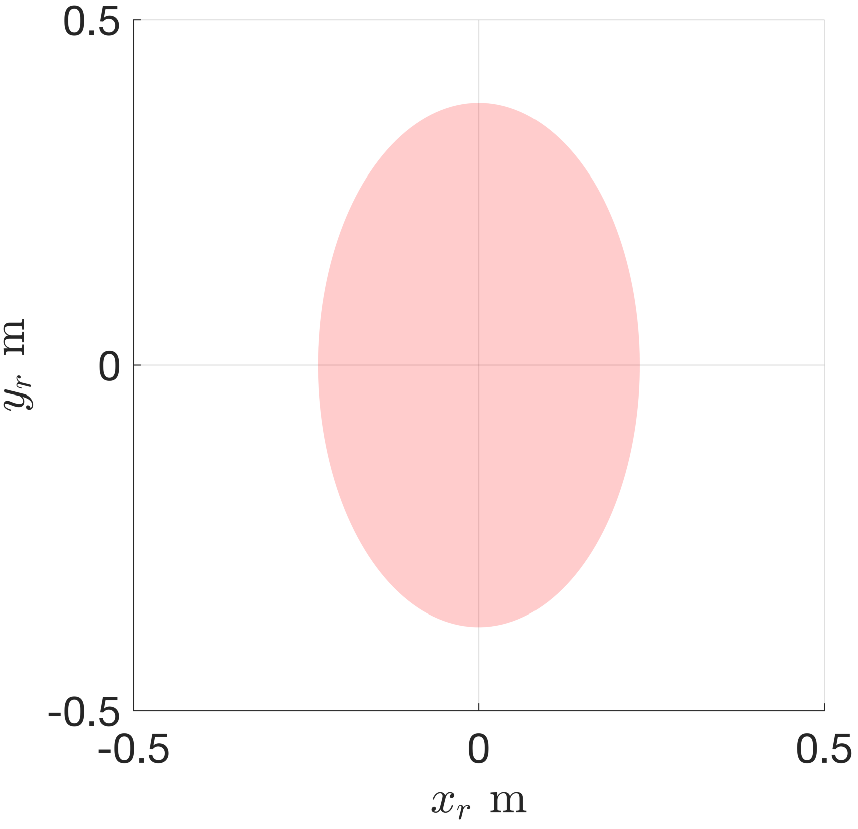
\includegraphics[width=0.3\textwidth]{5d/sos1.pdf} & 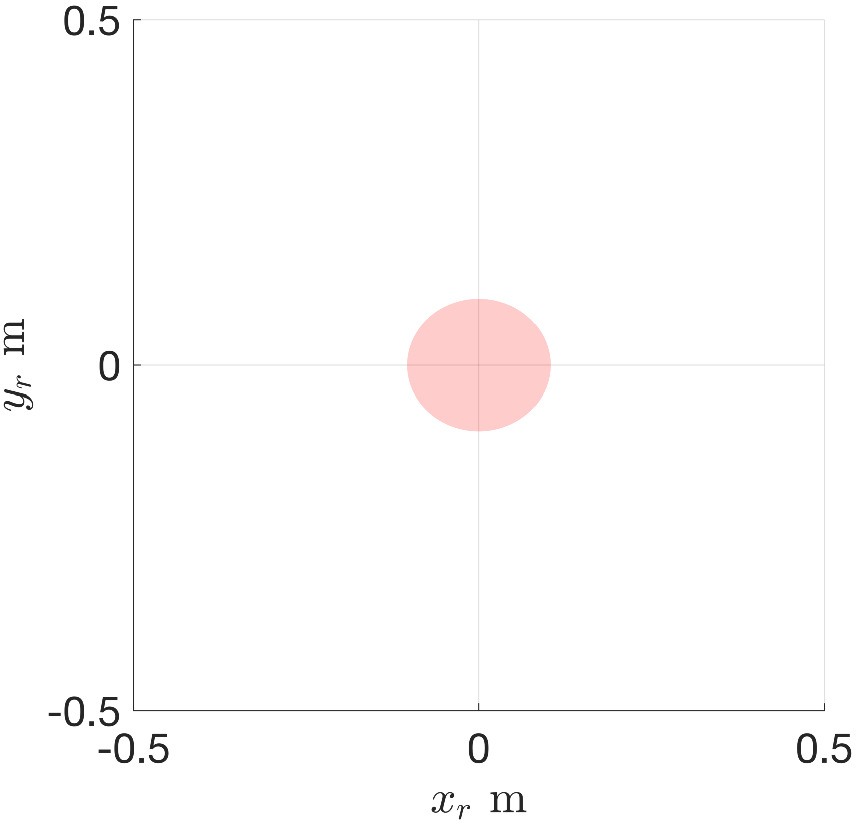
\includegraphics[width=0.3\textwidth]{5d/ellipse1.pdf}\\
		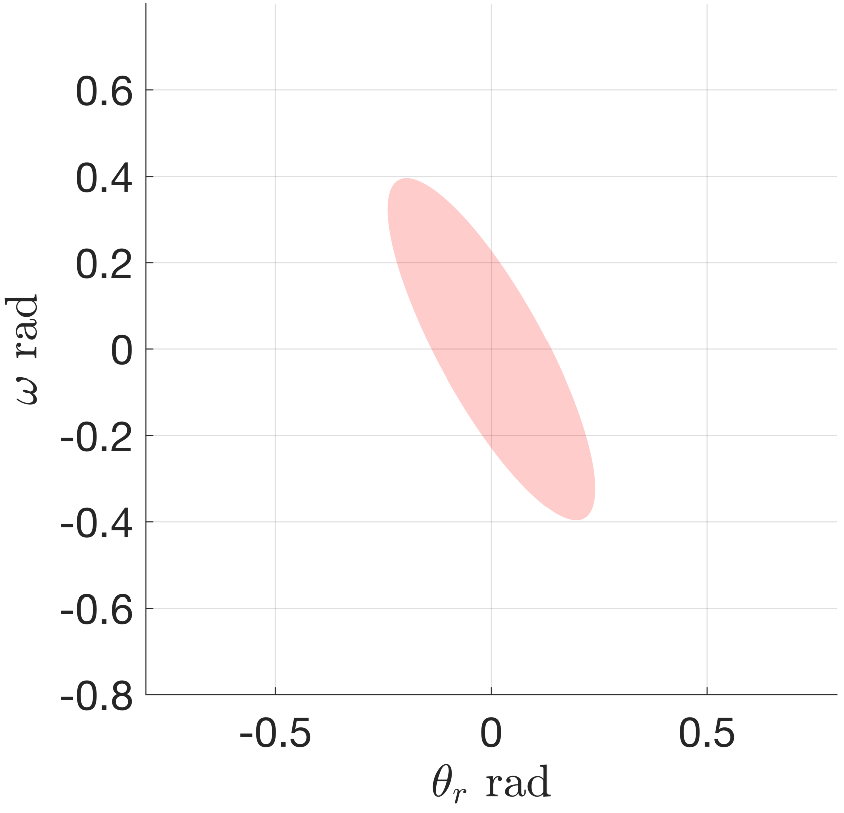
\includegraphics[width=0.3\textwidth]{5d/sos2.pdf} & 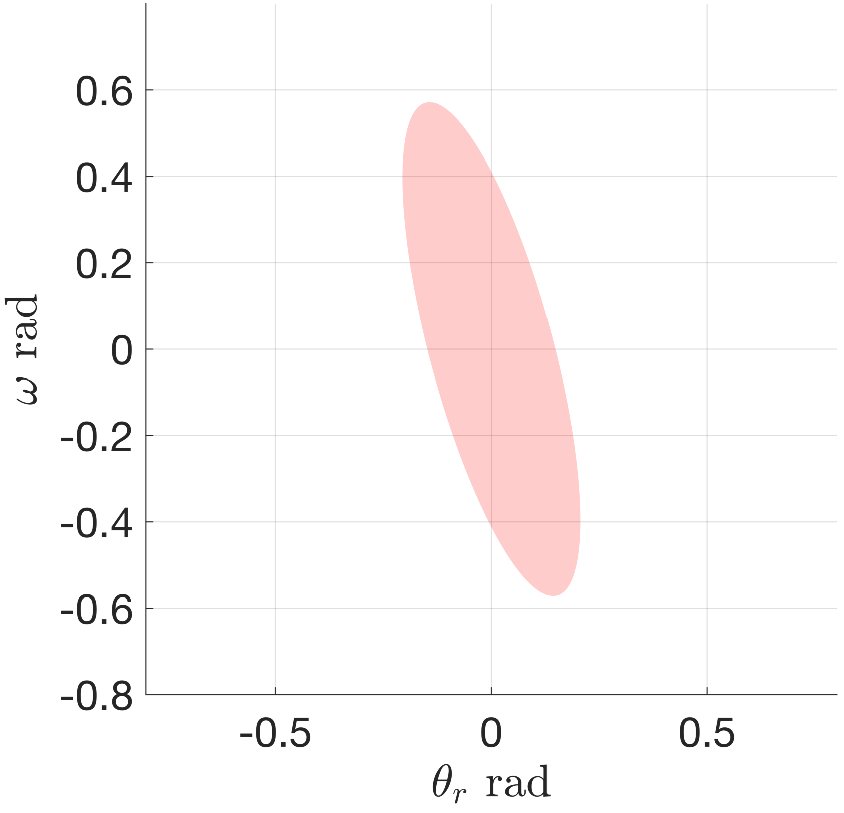
\includegraphics[width=0.3\textwidth]{5d/ellipse2.pdf}\\
		\hline
	\end{tabular}
	\caption{The minimum error bounds that SOS based algorithm finds on $x_r$, $y_r$ and $\theta_r$ are about 0.25 m, 0.35m and 0.25 rad. Setting the safety constraint to be within this box, the ellipsoidal CInvS algorithm is able to find a CInvS, and the tracking error could be a lot less. In fact, the box can be set to be even smaller, and we can still find an ellipsoidal CInvS.}
	\label{5d-compare}
\end{table}

\begin{table}[H]
	\centering
	\begin{tabular}{|c|c|}
		\hline
		\makecell{SOS based control\\Lyapunov function method \cite{sos-tracking}}  & \makecell{Ellipsoidal CInvS\\$\Delta t = 0.1$s}\\
		\hline
		73.068 s & 0.057 s \\
		\hline
	\end{tabular}
	\caption{Run time for each algorithm. For fair comparison, the disturbance and control are set to be the same. The safety constraint in ellipsoidal CInvS are set to be the minimum error bound achieved by the SOS based algorithm.}
	\label{5d-runtime}
\end{table}

In addition, the SOS based method is very fragile. It requires complex parameter tuning and a very careful initial guess of the bounding set. My algorithm is much robust, and we can throw a system and set of disturbance to the algorithm, without tuning and waiting.

\subsection{Future works for CInvS of nonlinear systems}
\begin{enumerate}
	\item Handling more complex nonlinear systems, such as coupled terms.
	\item Write a real time nonlinear MPC solver, verify the calculated CInvS is indeed one CInvS.
	\item Robust RRT for nonlinear system using control post for planning?
	\item Robust LQR for nonlinear system?
\end{enumerate}


\begin{thebibliography}{9}

\bibitem{correct-by-construction} 
Nilsson, Petter, et al. "Preliminary results on correct-by-construction control software synthesis for adaptive cruise control." Decision and Control (CDC), 2014 IEEE 53rd Annual Conference on. IEEE, 2014.

\bibitem{lk-cinvs} 
S. Smith, P. Nilsson, and N. Ozay.
Interdependence quantification for compositional control synthesis: An application in vehicle safety systems in IEEE CDC, 2016

\bibitem{control-barrier} 
Xu, Xiangru, et al.
Correctness guarantees for the composition of lane keeping and adaptive cruise control.
IEEE Transactions on Automation Science and Engineering15.3 (2018): 1216-1229.

\bibitem{sos-tracking}
Singh, Sumeet, et al. 
Robust Tracking with Model Mismatch for Fast and Safe Planning: an SOS Optimization Approach.
arXiv preprint arXiv:1808.00649 (2018).

\bibitem{ellipsoid-toolbox}
Kurzhanskiy, Alex A., and Pravin Varaiya.
Ellipsoidal toolbox (ET).
Proceedings of the 45th IEEE Conference on Decision and Control. IEEE, 2006.

\bibitem{ellipsoidal-calculus}
Kurzhanskiĭ, A. B., and István Vályi. Ellipsoidal calculus for estimation and control. Nelson Thornes, 1997.

\bibitem{control-tube}
Kurzhanski, Alexander B. "Dynamics and control of trajectory tubes. Theory and computation." 2014 20th International Workshop on Beam Dynamics and Optimization (BDO). IEEE, 2014.

\bibitem{convexopti}
Boyd, Stephen, and Lieven Vandenberghe. Convex optimization. Cambridge university press, 2004.

\bibitem{ecos}
Alexander Domahidi, Eric Chu, Stephen Boyd. "ecos: An Embedded
Conic Solver." In proceedings of European Control Conference (ECC), 
pp. 3071-3076, Zurich, Switzerland, July 2013."

\end{thebibliography}

\end{document}
